\chapter{Release 3 : Workflow du Budget Non-Industriel (Sprint 4)}
\label{chap:sprint_4}

\section{Introduction}
Les précédents sprints ont permis de maîtriser la capacité de production liée directement au produit automobile (machines de coupe, surface d'assemblage). Toutefois, le bon fonctionnement d'une usine COFAT dépend également d'un écosystème d'investissements dits "non-industriels" : modernisation de l'infrastructure informatique (IT), aménagement des bâtiments (Building), ou achats logistiques. La gestion de ce budget, traditionnellement réalisée par des allers-retours de courriels sans traçabilité, nécessitait une digitalisation urgente. Ce cinquième chapitre, couvrant le Sprint 4 (Release 3), clôture la réalisation technique du projet. Nous commencerons par définir les objectifs et la complexité technique de ce sprint, modélisés à travers le backlog spécifique. Ensuite, nous détaillerons le workflow collaboratif budgétaire implémenté, en insistant sur le rôle volontairement restreint de l'Acheteur (Achat) et l'absence d'étape de validation contraignante par l'Administrateur. Le mécanisme de notifications en temps réel, garantissant la fluidité des échanges, sera expliqué d'un point de vue backend (Node.js). Enfin, nous présenterons les fonctionnalités d'exportation (Excel/PDF) destinées à la direction et analyserons l'interface utilisateur finalisée.

\section{Objectifs et complexité du Sprint 4}
Le développement d'un workflow financier au sein d'une SPA (Single Page Application) est techniquement plus ardu que la simple manipulation de données. Ce sprint intègre une forte logique d'état asynchrone entre différents profils d'utilisateurs. 

Les objectifs fixés avec le Product Owner étaient les suivants :
\begin{enumerate}
    \item Permettre la création et la soumission de demandes de budget non-industriel structurées par département.
    \item Implémenter un tunnel de modification stricte des prix par le département Achat, avec un recalcul automatique côté serveur.
    \item Assurer une traçabilité des modifications via un système d'alerte (notifications) instantané.
    \item Générer des rapports binaires professionnels téléchargeables (exports).
\end{enumerate}

\textbf{Modèles de données impliqués :}
Pour soutenir ces objectifs, deux modèles Sequelize majeurs ont été implémentés dans la base SQL Server :
\begin{itemize}
    \item \textbf{\texttt{NonIndustrialBudget}} : Stocke la demande financière. Ses champs réels sont \texttt{department} (IT, HR, QUALITY, BUILDING, LOGISTICS, MAINTENANCE, PRODUCTION), \texttt{area}, \texttt{equipment}, \texttt{qty}, \texttt{currency}, \texttt{unitPrice}, \texttt{totalPrice} (calculé par hook), \texttt{createdBy}, et \texttt{updatedBy}.
    \item \textbf{\texttt{BudgetNotification}} : Stocke la piste d'audit et les messages. Ses champs sont \texttt{type} (NEW\_REQUEST, PRICE\_UPDATED), \texttt{message}, \texttt{isRead}, \texttt{budgetItemId}, \texttt{fromUser}, \texttt{toRole}, et \texttt{toUser}.
\end{itemize}

\section{Backlog du Sprint 4}
Le tableau \ref{tab:backlog_sprint4} récapitule les User Stories développées durant ce mois d'août 2026. La complexité de ce sprint ne résidait pas dans les interfaces graphiques, mais dans la synchronisation de l'état React entre les sessions parallèles du Site Manager et de l'Acheteur, ainsi que dans la génération de fichiers binaires (PDF/XLSX) côté serveur Node.js.

\begin{table}[h]
\centering
\begin{tabular}{|p{2cm}|p{8cm}|p{2cm}|p{2cm}|}
\hline
\textbf{ID US} & \textbf{Description} & \textbf{Acteur} & \textbf{Complexité} \\ \hline
US-11 & En tant que Site Manager, je veux saisir et soumettre des lignes de budget avec recalcul auto du total. & Site Mgr & Moyenne \\ \hline
US-12 & En tant qu'acheteur, je veux modifier les prix/devises des demandes soumises. & Achat & Haute \\ \hline
US-13 & En tant qu'utilisateur, je veux voir une cloche de notification se mettre à jour lors d'une action budgétaire. & Tous & Haute \\ \hline
US-14 & En tant que Site Manager ou Acheteur, je veux exporter le tableau budgétaire au format Excel ou PDF. & Tous & Moyenne \\ \hline
\end{tabular}
\caption{Backlog spécifique du Sprint 4}
\label{tab:backlog_sprint4}
\end{table}

\section{Le Workflow Budgétaire : Scénario et Permissions}
Le processus métier de demande de budget chez COFAT a été modélisé pour être extrêmement agile. Contrairement aux lourds systèmes ERP (comme SAP) où chaque étape nécessite l'approbation hiérarchique d'un administrateur, notre système privilégie l'action directe. \textbf{Il n'y a aucune étape de validation/rejet formelle par l'Administrateur dans ce workflow}. L'Administrateur surveille, mais n'interfère pas.

\textbf{Le scénario réel se déroule en trois étapes fluides :}

\begin{table}[h]
\centering
\begin{tabular}{|p{2cm}|p{3.5cm}|p{9.5cm}|}
\hline
\textbf{Étape} & \textbf{Acteur actif} & \textbf{Action métier et réaction du système} \\ \hline
\textbf{1. Création} & Site Manager (Demandeur) & Saisie d'une nouvelle ligne de budget via le formulaire de son usine. Il indique le \textit{Department} (ex: IT), l'\textit{Equipment} (ex: Serveur Dell), la \textit{Quantity} et son estimation de prix. La ligne prend le statut initial de brouillon ("Draft"). \\ \hline
\textbf{2. Soumission} & Site Manager & Soumission de la ligne. Le statut passe à "Submitted". Le backend enregistre la demande et génère automatiquement un événement \texttt{NEW\_REQUEST}. \\ \hline
\textbf{3. Édition du Prix} & Acheteur (Achat) & L'Achat se connecte, ouvre la liste des demandes "Submitted". S'il a obtenu un devis fournisseur meilleur marché, il \textbf{modifie uniquement le coût unitaire (unit price) et la devise (currency)}. C'est l'unique action que ce rôle peut effectuer sur la demande. \textbf{Le backend recalcule instantanément le \textit{total price}} ($Qty \times UnitPrice$). L'action fait avancer la demande sans aucune validation d'un tiers. \\ \hline
\end{tabular}
\caption{Déroulement du workflow du budget non-industriel}
\label{tab:workflow_budget}
\end{table}

\textbf{Sécurité de la logique métier côté serveur :} 
Dans le code source Express (\texttt{routers/nonIndustrialBudgetRoutes.js}), la restriction du rôle Achat est strictement implémentée lors d'une requête \texttt{PUT /update/:id}. Si le JWT contient \texttt{userRole === 'Achat'}, l'algorithme ignore toute tentative de modification de la quantité ou de la description de l'équipement, et n'autorise l'enregistrement que des champs \texttt{currency} et \texttt{unitPrice}.

\section{Système de Notifications Temps Réel}
Pour remplacer les échanges d'emails asynchrones et informels, le système intègre un moteur de notification intra-applicatif robuste.

\textbf{Mécanisme technique :}
Le serveur Express possède un module \texttt{budgetNotificationHelper.js}. Chaque fois qu'une action budgétaire est interceptée (par exemple, la route POST de création ou la route PUT de mise à jour des prix), une ligne est insérée dans la table \texttt{BudgetNotification}.
\begin{itemize}
    \item Si l'Achat met à jour un prix, le système crée une notification de type \texttt{PRICE\_UPDATED} avec un message textuel décrivant la baisse ou la hausse tarifaire, dirigée spécifiquement vers le \texttt{Site Manager} qui avait créé la ligne (\texttt{toRole: 'User', toUser: budget.createdBy}).
    \item Si un Site Manager modifie sa demande, l'alerte (\texttt{REQUEST\_MODIFIED}) est envoyée vers le groupe \texttt{toRole: 'Achat'}.
\end{itemize}

Côté client React, une icône "Cloche" dans la barre de navigation effectue un \textit{polling} (requêtes GET vers \texttt{/api/non-industrial-budget/notifications/unread} pour le budget, ou \texttt{/api/notifications?unread\_only=true} pour les alertes générales) pour récupérer le compteur. Au clic, les messages s'affichent et une requête HTTP \texttt{PUT} (\texttt{/api/non-industrial-budget/notifications/:id/read} ou \texttt{/api/notifications/mark-read}) marque les alertes correspondantes comme lues dans la base de données.

\section{Exportation (Excel et PDF)}
Lors des réunions du Comité de Direction, le besoin d'extraire la donnée du système pour en faire des présentations est indispensable. L'US-14 permet l'exportation des tableaux.

\textbf{Export Excel :}
L'export Excel repose sur la bibliothèque \texttt{xlsx} (SheetJS), disponible à la fois côté serveur Node.js (via \texttt{utils/excelImporter.js}, qui implémente \texttt{exportBudgetToExcel}) et côté navigateur (composants React). Dans le module Budget Non-Industriel, l'export est généré directement dans le navigateur via le composant \texttt{NonIndustrialBudgetImproved.js} :
1. Les données du tableau sont transformées en tableau d'objets JSON.
2. La bibliothèque \texttt{xlsx} crée un classeur (\textit{workbook}) en mémoire avec les colonnes : \textbf{N\textdegree, Department, Area, Equipment, QTY, Currency, Unit Price, Total Price}.
3. Le fichier est téléchargé directement par le navigateur via la méthode \texttt{XLSX.writeFile()}.

\textbf{Export PDF :}
L'export PDF est également généré côté client (navigateur) à l'aide des bibliothèques \texttt{jspdf} et \texttt{jspdf-autotable}, disponibles dans le \texttt{package.json} frontend. Le composant React génère le document PDF en mémoire, formatant les données en tableau avec l'en-tête COFAT, la date et les récapitulatifs financiers, avant de déclencher le téléchargement via \texttt{doc.save()}. Ce choix technique de génération côté client allège la charge du serveur Node.js.

\section{Réalisation du Sprint 4 : Analyse de l'interface}
L'aboutissement de cette architecture asynchrone se concrétise dans une interface moderne et hautement réactive, développée en React/MUI/Tailwind.

\vspace{0.5cm}
\begin{figure}[H]
    \centering
    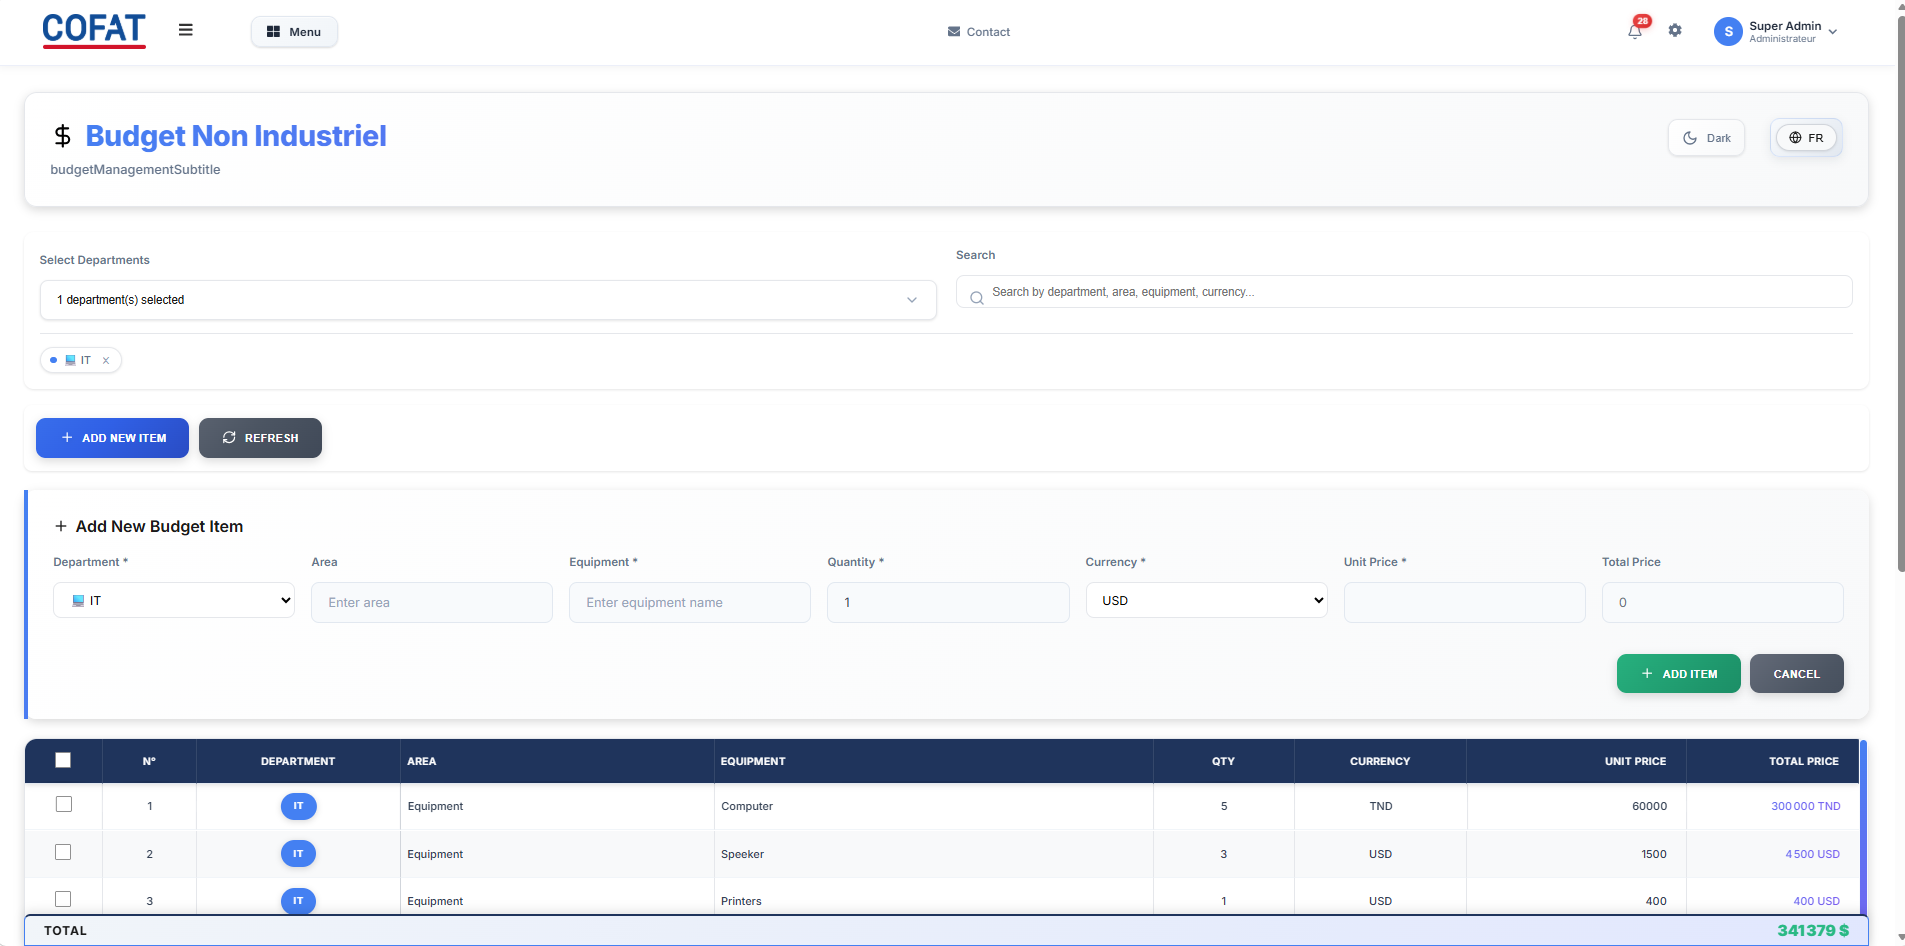
\includegraphics[width=1\textwidth]{img/non industrial budget.png}
    \caption{Interface de gestion dynamique du budget non-industriel}
    \label{fig:non_industrial_budget}
\end{figure}
\vspace{0.5cm}

\textbf{Description de l'interface métier (Figure \ref{fig:non_industrial_budget}) :}
L'écran principal de budgétisation présente un tableau de données exhaustif et dynamique. L'utilisateur y retrouve les colonnes précitées (N°, DEPARTMENT, AREA, EQUIPMENT, QTY, CURRENCY [TND/USD/EUR/MXN/BRL], UNIT PRICE, TOTAL PRICE). 
La particularité de cet écran réside dans son formulaire d'ajout \textit{inline} (visible sur la capture), permettant de saisir une nouvelle ligne directement au-dessus du tableau sans ouvrir de fenêtre modale intrusive. Des boutons d'action rapides (\textbf{ADD NEW ITEM}, \textbf{REFRESH}) trônent au sommet. Fait notable : le système calcule et maintient en temps réel la \textbf{ligne de TOTAL cumulatif} visible en bas de la grille, adaptant la somme à chaque filtre appliqué ou modification de prix validée par l'Acheteur.

\vspace{0.5cm}
\begin{figure}[H]
    \centering
    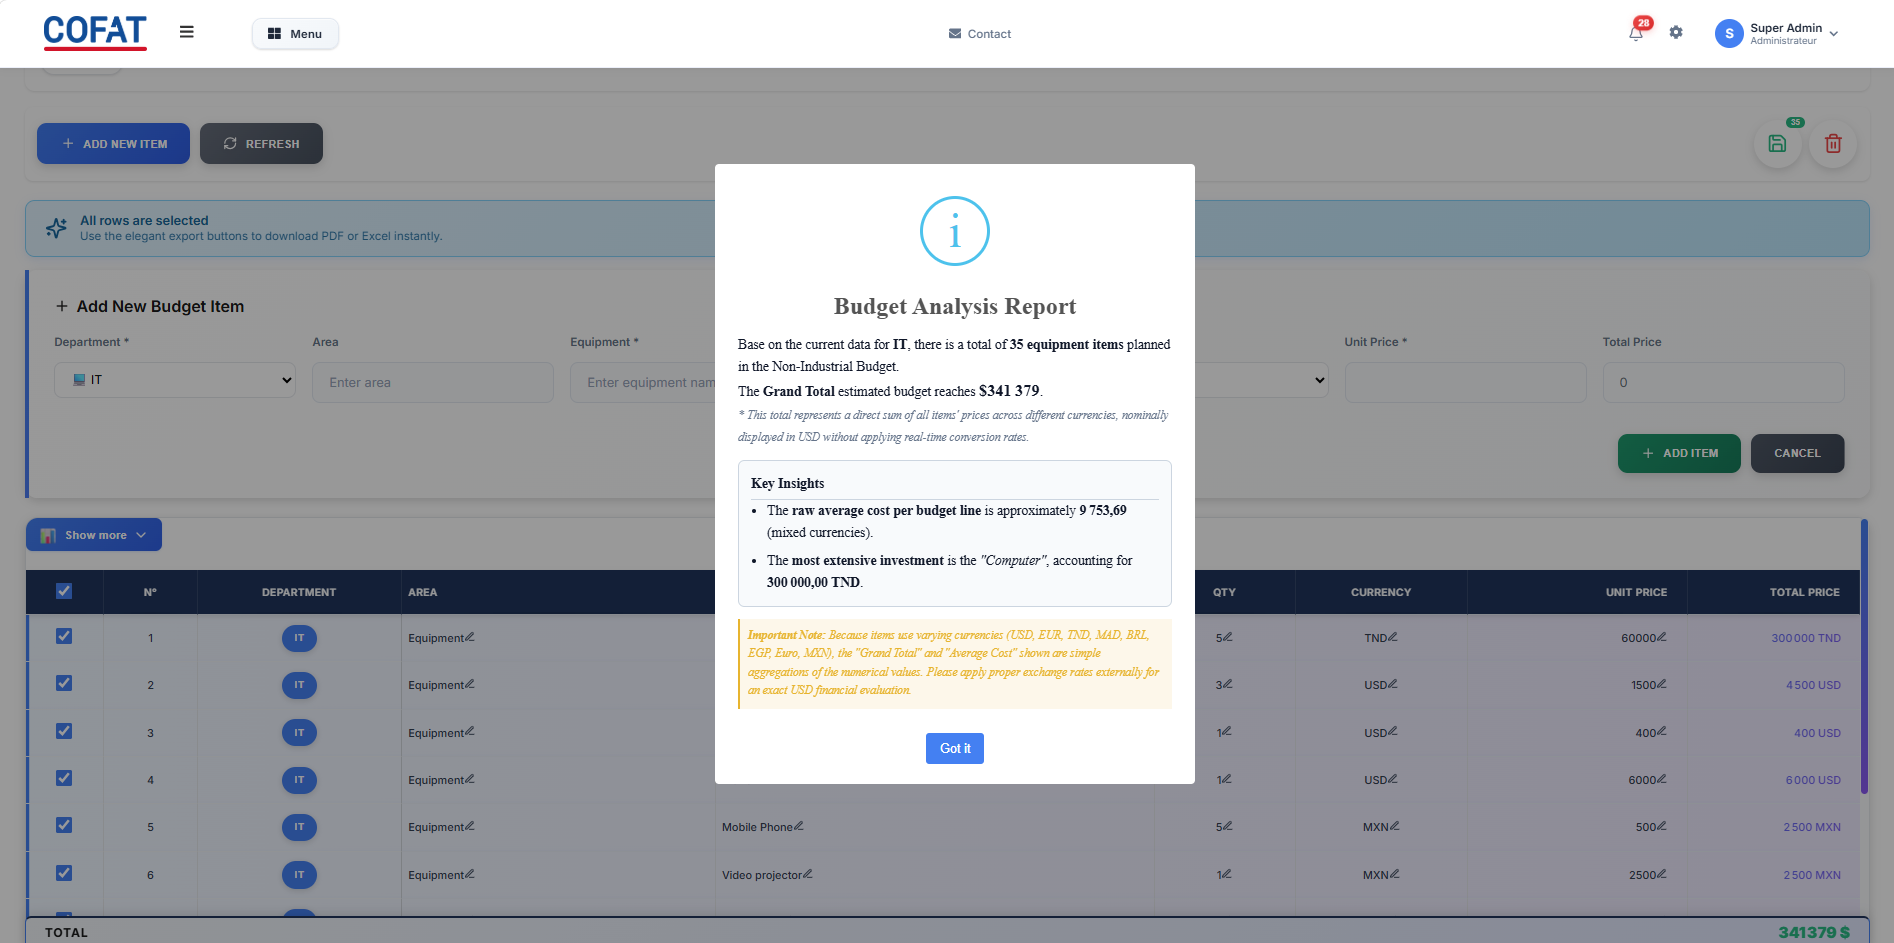
\includegraphics[width=0.9\textwidth]{img/non industrial budget analyse.png}
    \caption{Tableau de bord d'analyse des dépenses par département}
    \label{fig:analyse_budget}
\end{figure}
\vspace{0.5cm}

Afin d'accompagner la validation globale du budget au niveau corporatif, l'interface propose un onglet analytique (Figure \ref{fig:analyse_budget}). Les graphiques (Charts.js) générés par le backend (\texttt{GET /stats/by-department}) ventilent les dépenses non-industrielles par grand département (IT, Qualité, Bâtiment). Le directeur financier de COFAT peut ainsi visualiser immédiatement, via un graphique en anneau (Doughnut chart) et un histogramme par devises, si le budget IT mondial dépasse l'enveloppe allouée pour l'année.

\section{Conclusion}
Le Sprint 4 a couronné le succès du projet en intégrant la dimension financière à la gestion capacitaire. L'ingénierie mise en place dans le workflow du budget non-industriel prouve la maturité de l'architecture Node.js/React : gestion fine des droits RBAC (restreignant chirurgicalement l'Achat à la modification tarifaire), recalculs automatiques par l'ORM Sequelize, moteur de notification intra-applicatif et génération de rapports Excel/PDF serveur. Ces fonctionnalités mettent un terme définitif à la perte de traçabilité et aux lourdeurs bureaucratiques des processus antérieurs. L'application \textit{Cofat Capacity Study} est désormais complète, opérationnelle, et prête à soutenir la stratégie de croissance globale du Groupe COFAT.
